\chapter[Introdução]{Introdução}
% \addcontentsline{toc}{chapter}{Introdução}

Segundo \citeonline{violence_against_women}, o termo violência contra a mulher trata de
diversos atos de abuso e violência baseados no gênero, ou seja, dirigidos à mulheres e meninas ao longo da vida.
Para \citeonline{violence_global}, dos diversos tipos de violência existentes, a violência doméstica, ou proveniente do parceiro,
e a violência sexual, proveniente de um indivíduo diferente do parceiro, são as formas de violência que prevalecem.

A pesquisa relatada por \citeonline{violence_global} mostra que 35\% das mulheres no mundo já vivenciaram uma situação
de violência pelo física e/ou sexual pelo parceiro e violência sexual por outro indivíduo. No mundo, 38\% dos homicídios de mulheres são cometidos pelos parceiros das vítimas.

No Brasil, de acordo com o Sistema de Informações sobre Mortalidade (SIM), entre 1980 e 2013, 106.093 mulheres foram vítimas de homicídio, representando em 2013 uma taxa de aproximadamente 13 homicídios femininos
diários \cite{mapa_violencia_2015}. 
No primeiro semestre de 2016 foram contabilizados 555.634 atendimentos na central de denúncias 
de violência contra a mulher, de acordo com o levantamento feito pela Secretaria de Políticas para as Mulheres (SPM). 
Aproximadamente 54\% dos atendimentos foram para prestação de informações. De acordo com \cite{portal_180}, aproximadamente 13\% dos atendimentos, são relatos de violência física (51\%), psicológica (31,1\%), moral (6,51\%), patrimonial (1,93\%), sexual (4,30\%), cárcere privado (4,86\%) e tráfico de pessoas (0,24\%).

Ao longo dos anos, cenários como esse impulsionaram os governos à criação de políticas públicas (PP) para a redução da violência contra as mulheres e de estratégias de apoio às mulheres e de conscientização da população. Além disso, estratégias tecnológicas, como aplicativos e sites, têm surgido nesse contexto.

O I-DECIDE é um projeto australiano, proveniente dessas estratégias, responsável por disponibilizar para as mulheres um site
no qual elas podem avaliar sua relação, suas prioridades e planejar um futuro mais seguro. A ferramenta compreende avaliações de segurança e um processo de planejamento de ação individualizado adaptado às circunstâncias particulares de cada mulher. \footnote{Traduzido de I-DECIDE: Trial of an online healthy relationship tool and safety decision aid for women experiencing domestic violence - http://medicine.unimelb.edu.au/research-groups/general-practice-research/abuse-and-violence/development-and-evaluation-of-an-online-healthy-relationship-tool-and-safety-decision-aid-for-women-experiencing-domestic-violence-i-decide}

No Brasil, a criação da Lei Maria da Penha, da Lei do Feminicídio e de programas e serviços de apoio à causa 
como o Disque-denúncia Ligue 180, a Casa da Mulher Brasileira e a Unidade Móvel de Atendimento são respostas aos cenários supracitados. No contexto de Tecnologia da Informação (TI), a criação de software têm sido apoiada pelo governo e realizada pela própria população.

Em 2011, o Laboratório Hacker da Câmara dos Deputados promoveu um \textit{Hackathon} de Gênero e Cidadania, no qual
um dos temas era "Violência Contra a Mulher". O site Minha Voz foi o vencedor e de suas funcionalidades é um questionário que ajuda a mulher a identificar o tipo de violência sofrida. 

Na Figura \ref{fig:sistemas_categorizados} são apresentadas algumas aplicações criadas no Brasil para apoio à mulher vítima de violência categorizadas em cinco tipos: Levantamento de Dados e estatísticas, Mapeamento de riscos, Informativos, Pedido de Socorro e Apoio.

\begin{figure}[ht]
\centering
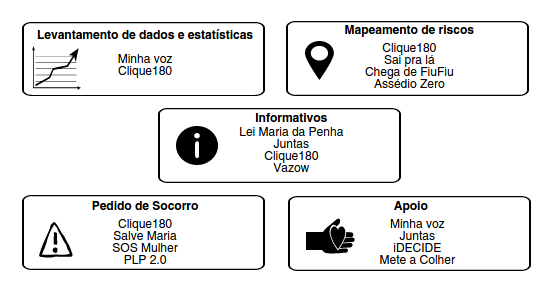
\includegraphics[scale=0.85]{figuras/sistemas_relacionados.png}
\caption{Aplicações de apoio à mulher vítima de violência}
\label{fig:sistemas_categorizados}
\end{figure}

Em suma, os sistemas estão voltados para informações, pedido de socorro e uma rede de desabafo e apoio entre as mulheres. 
As aplicações classificadas como apoio, no geral apresentam informações genéricas sobre como agir em situações de violência. Dessa forma, percebe-se uma lacuna em um apoio mais específico de acordo com a situação de violência, como sugestões de ações a serem tomadas e planejamento de segurança, como por exemplo, a proposta do I-DECIDE.

\section{Objetivo}

Considerando a lacuna identificada nos sistemas existentes, o objetivo do trabalho é 
criar uma \textit{Application Programming Interface} (API) para uso em sistemas de tomada de 
decisão e planejamento de segurança para mulheres vítima de violência, utilizando o modelo definido e utilizado na aplicação I-DECIDE.
Para esse fim os objetivos específicos do trabalho são:
\begin{itemize}
	\item Definir um questionário padrão a ser respondido pelas mulheres para apoio a tomada de decisão;
	\item Permitir que novas questões sejam inseridas pelas mulheres;
	\item Categorizar as questões (padrão e inseridas);
	\item Definir ações de segurança para as categorias de violência;
\end{itemize}

\section{Metodologia}








